\begin{proofbox}
\textbf{证明一：门槛最低——初中面积、相似和线段比例（推荐先读）}

\textbf{目标：}先只用初中几何弄清 $I$ 如何定位，再把结果改写为高中向量语言。\textbf{前面第 1--6 步无需向量知识。}
\VIncenterFigure{1}{.5}{14}{15}{13}{先看三块同高面积：共同的高为 $r$，所以三块面积与各自底边 $a,b,c$ 成比例。}
\begin{enumerate}
\item \textbf{画辅助线：} 在三角形内连接 $IA,IB,IC$，从 $I$ 分别向三边作垂线。因为 $I$ 是内切圆圆心，三条垂线都长 $r$。
\item \textbf{分出三块面积：}由“面积等于底乘高的一半”，
\[
S_{IBC}=\frac{ar}{2},\quad S_{ICA}=\frac{br}{2},\quad S_{IAB}=\frac{cr}{2}.
\]
所以 $S_{ABC}=r(a+b+c)/2$，并有
\[
\frac{S_{IBC}}{S_{ABC}}=\frac{a}{a+b+c}.
\]
\item \textbf{找第一个分点 $D$：}延长直线 $AI$ 交边 $BC$ 于 $D$。由于 $AI$ 平分 $\angle BAC$，初中角平分线定理给出
\[
\frac{BD}{DC}=\frac{AB}{AC}=\frac cb,
\quad\Longrightarrow\quad \frac{BD}{BC}=\frac{c}{b+c}.
\]
这里 $BC=BD+DC$，因此最后一个分数分母是 $b+c$，不是 $a$。
\item \textbf{确定 $I$ 在 $AD$ 上的位置：}三角形 $IBC$ 与 $ABC$ 有同一条底边 $BC$，面积之比就是从 $I$、$A$ 到直线 $BC$ 的高之比。因为 $A,I,D$ 在一条直线上，且 $D\in BC$，从 $A,I$ 向 $BC$ 作垂线所得的两个直角三角形相似，所以两条高之比是 $DI:DA$。因此
\[
\frac{DI}{DA}=\frac{S_{IBC}}{S_{ABC}}=\frac{a}{a+b+c},
\qquad
\frac{AI}{AD}=1-\frac{DI}{AD}=\frac{b+c}{a+b+c}.
\]
\VIncenterFigure{3}{.57}{14}{15}{13}{$AH\parallel IK$，$A,I,D$ 共线，所以 $\triangle DAH\sim\triangle DIK$；同底面积比等于 $IK/AH=DI/DA$。}
这一步不需要余弦定理，也不需要求任何角的大小。
\item \textbf{用初中坐标方法找 $D$：}假设 $B(x_2,y_2),C(x_3,y_3)$。$D$ 从 $B$ 向 $C$ 走了 $\frac{c}{b+c}$ 段，因此
\[
\begin{aligned}
x_D&=x_2+\frac{c}{b+c}(x_3-x_2)=\frac{bx_2+cx_3}{b+c},\\
y_D&=y_2+\frac{c}{b+c}(y_3-y_2)=\frac{by_2+cy_3}{b+c}.
\end{aligned}
\]
\item \textbf{再用坐标比例找 $I$：}点 $I$ 从 $A$ 向 $D$ 走了 $\frac{b+c}{a+b+c}$ 段。因此
\[
\begin{aligned}
x_I&=x_1+\frac{b+c}{a+b+c}(x_D-x_1)
=\frac{ax_1+bx_2+cx_3}{a+b+c},\\
y_I&=y_1+\frac{b+c}{a+b+c}(y_D-y_1)
=\frac{ay_1+by_2+cy_3}{a+b+c}.
\end{aligned}
\]
至此，\textbf{已用初中几何、线段比例与坐标运算得出内心坐标}。
\item \textbf{最后才翻译成高中向量：} 对任意参考点 $O$，上面两行坐标等式可以合写为
\[
(a+b+c)\vec{OI}=a\vec{OA}+b\vec{OB}+c\vec{OC}.
\]
由 $\vec{OA}=\vec{OI}+\vec{IA}$（另两项同理），移项并约去 $(a+b+c)\vec{OI}$，得到
\[
\boxed{a\vec{IA}+b\vec{IB}+c\vec{IC}=\vec0}.
\]
\end{enumerate}
\textbf{这一法的收获：}三个系数不是凭空出现，而是由相同的高、面积比和两次线段比例自然推出。
\end{proofbox}

\begin{proofbox}
\textbf{证明二：步骤最少——利用三块面积直接定位（考场短证明）}

\textbf{先说明所用的小结论：}若点 $P$ 在 $\triangle ABC$ 内，把三个小三角形面积记为
$U=S_{PBC},\ V=S_{PCA},\ W=S_{PAB}$，则
% P is deliberately not the incenter. A=(5,12),B=(0,0),C=(14,0),P=(6,5).
\begin{center}
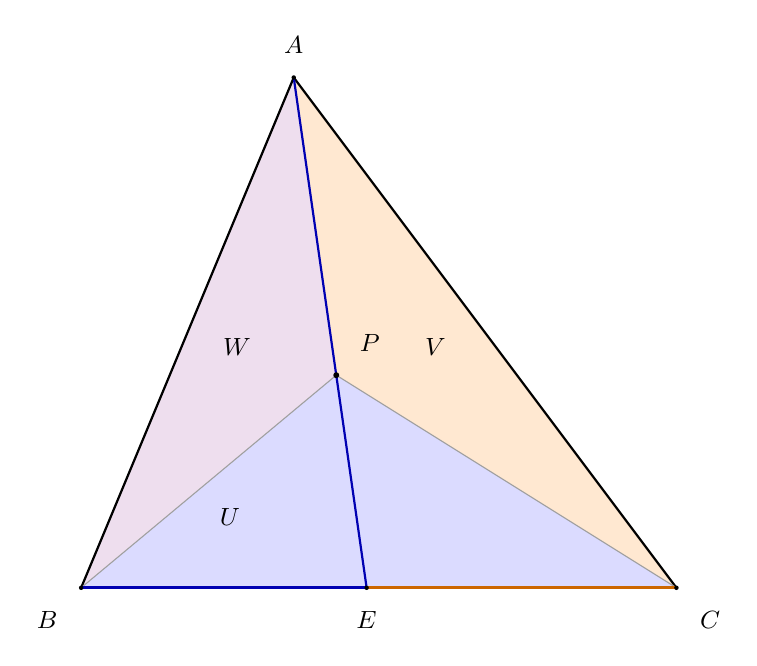
\begin{tikzpicture}[scale=.54,font=\small,line cap=round,line join=round]
\coordinate (A) at (5,12);\coordinate (B) at (0,0);\coordinate (C) at (14,0);
\coordinate (P) at (6,5);\coordinate (E) at (47/7,0);
\fill[blue!14] (P)--(B)--(C)--cycle;
\fill[orange!18] (P)--(C)--(A)--cycle;
\fill[violet!13] (P)--(A)--(B)--cycle;
\draw[thick] (A)--(B)--(C)--cycle;
\draw[gray!75] (P)--(B) (P)--(C);
\draw[thick,blue!70!black] (A)--(E);
\draw[blue!70!black,very thick] (B)--(E);
\draw[orange!80!black,very thick] (E)--(C);
\node at (3.5,5/3) {$U$};
\node at (25/3,17/3) {$V$};\node at (11/3,17/3) {$W$};
\foreach \Q/\pos in {A/above,B/below left,C/below right,E/below}{\fill (\Q) circle[radius=1.5pt];\node[\pos=5pt] at (\Q) {$\Q$};}
\fill (P) circle[radius=2pt];\node[above right=5pt] at (P) {$P$};
\end{tikzpicture}
\par\smallskip{\small $P$ 是任意内点；同高给出 $BE:EC=W:V$，同底给出 $PE:AE=U:(U+V+W)$。}
\end{center}

\[
\vec{OP}=\frac{U\vec{OA}+V\vec{OB}+W\vec{OC}}{U+V+W}.
\tag{*}
\]
\textbf{它为什么成立？} 令 $E=AP\cap BC$。$\triangle ABE$ 与 $\triangle ACE$ 对底边 $BE,EC$ 有同样的高，故面积比为 $BE:EC$。将顶点 $A$ 沿 $AE$ 移到 $P$，这两块面积都乘同一个比例 $AP/AE$，所以仍有 $BE:EC=W:V$。于是 $\vec{OE}=(V\vec{OB}+W\vec{OC})/(V+W)$。再由 $S_{PBC}/S_{ABC}=PE/AE=U/(U+V+W)$，有
$\vec{OP}=\bigl(U\vec{OA}+(V+W)\vec{OE}\bigr)/(U+V+W)$，代入即得 $(*)$。这里仅用了同高三角形面积比和线段按比例分点。

\textbf{正式证明只要两步：}
\begin{enumerate}
\item $I$ 到三边距离都为 $r$，故 $U:V:W=a:b:c$。
\item 将 $U:V:W=a:b:c$ 代入 $(*)$，立刻得到
\[
\vec{OI}=\frac{a\vec{OA}+b\vec{OB}+c\vec{OC}}{a+b+c}
\iff a\vec{IA}+b\vec{IB}+c\vec{IC}=\vec0.
\]
\end{enumerate}
\textbf{注意：}两步法\textbf{不是}不证明就套一个新定理；上面已给出面积定位式的初中理由。熟悉该理由后，考场可以简写。
\end{proofbox}

\begin{proofbox}
\textbf{证明三：常规方法——两次角平分线定理与向量分点}

这是教材常见的几何转向量路线；不必背“面积定位式”。
\VIncenterFigure{2}{.53}{14}{15}{13}{先在 $ABC$ 中用 $AD$，再在蓝色 $ABD$ 中用 $BI$；从 $I$ 指向 $A,D$ 的两个箭头反向。}
\begin{enumerate}
\item 令角平分线 $AI$ 与 $BC$ 相交于 $D$。角平分线定理给出
$BD:DC=AB:AC=c:b$，所以 $BD=ac/(b+c)$。
\item 因为 $I$ 是内心，$BI$ 也平分 $\angle ABC$。又因为 $D$ 在 $BC$ 上，$BI$ 也平分 $\angle ABD$。在 $\triangle ABD$ 中用角平分线定理：
\[
\frac{AI}{ID}=\frac{AB}{BD}=
\frac{b+c}{a}.
\]
图中的 $A,I,D$ 依次排列，两向量反向。
\item 由 $\vec{BC}=\vec{IC}-\vec{IB}$，以及 $BD/BC=c/(b+c)$，
\[
\begin{aligned}
\vec{ID}&=\vec{IB}+\vec{BD}=\vec{IB}+\frac{c}{b+c}(\vec{IC}-\vec{IB})\\
&=\frac{b\vec{IB}+c\vec{IC}}{b+c}.
\end{aligned}
\]
\item 因为 $AI/ID=(b+c)/a$ 且方向相反，
\[
\vec{IA}=-\frac{b+c}{a}\vec{ID}
=-\frac{b\vec{IB}+c\vec{IC}}{a}.
\]
两边同乘 $a$ 再移项：
\[\boxed{a\vec{IA}+b\vec{IB}+c\vec{IC}=\vec0}.\]
\item 对任意 $O$，代入 $\vec{IA}=\vec{OA}-\vec{OI}$（另两项同理），即得
$(a+b+c)\vec{OI}=a\vec{OA}+b\vec{OB}+c\vec{OC}$。
再取 $O$ 为坐标原点、分别比较横纵坐标，就得到内心坐标公式。
\end{enumerate}
\end{proofbox}

\begin{proofbox}
\textbf{证明四：独立验证——高中坐标与点到直线距离（适合检查公式）}

这个方法不借助角平分线定理，而是先用公式找出候选点 $P$，再验证它到三条边距离相等。
\begin{enumerate}
\item 取 $B(0,0)$、$C(a,0)$、$A(u,h)$，其中 $a>0,h>0$。两条斜边为
\[
b=AC=\sqrt{(u-a)^2+h^2},\quad
c=AB=\sqrt{u^2+h^2}.
\]
设 $L=a+b+c$，并定义
\[
P=\frac{aA+bB+cC}{L}
=\left(\frac{a(u+c)}{L},\frac{ah}{L}\right).
\]
这里等式只是在横、纵坐标上分别加减乘除。
\VIncenterFigure{4}{.49}{14}{15}{13}{蓝色线段是候选点 $P$ 到三边的垂直距离；逐一算出均为 $ah/L$，再核对 $P$ 位于内部。}
\item 到底边 $BC$（即 $y=0$）的距离为
\[d(P,BC)=\frac{ah}{L}.\]
\item 直线 $AB$ 过 $B(0,0)$ 和 $A(u,h)$，方程为 $hx-uy=0$；其法向量长度为 $\sqrt{h^2+u^2}=c$。代入点到直线距离公式：
\[
\begin{aligned}
d(P,AB)&=\frac{\left|h\cdot\frac{a(u+c)}L-u\cdot\frac{ah}L\right|}{c}
=\frac{ach/L}{c}=\frac{ah}{L}.
\end{aligned}
\]
\item 直线 $AC$ 的方程是 $h(x-a)-(u-a)y=0$，它的法向量长度为 $b$。所以
\[
\begin{aligned}
d(P,AC)&=\frac{\left|h\left(\frac{a(u+c)}L-a\right)-(u-a)\frac{ah}L\right|}{b}\\
&=\frac{|ah(c+a-L)/L|}{b}
=\frac{|{-abh/L}|}{b}=\frac{ah}{L}.
\end{aligned}
\]
\item $P$ 位于三角形内部：先在 $BC$ 上取 $D$，使
$\vec{OD}=(b\vec{OB}+c\vec{OC})/(b+c)$；因为 $b,c>0$，$D$ 在 $B,C$ 之间。再有
$\vec{OP}=(a\vec{OA}+(b+c)\vec{OD})/L$，故 $P$ 在 $A,D$ 之间。\textbf{内部}的 $P$ 到三边等距，因此它在三个内角平分线上，即 $P=I$。
\end{enumerate}
\textbf{适用价值：}它能独立核对公式，也提醒我们必须确认点在三角形内部；仅仅到三条\emph{直线}距离相等还可能得到三角形外部的其他等距点。
\end{proofbox}

\begin{proofbox}
\textbf{附证：原文件两条常用辅助公式为何成立}
\begin{enumerate}
\item \textbf{角平分线向量公式。}由 $BD:DC=c:b$，先写 $\vec{BD}=\frac c{b+c}\vec{BC}$，再用 $\vec{BC}=\vec{AC}-\vec{AB}$，得到
% M=A+b/(b+c)(B-A), N=A+c/(b+c)(C-A); A,M,D,N is a parallelogram.
\begin{center}
\begin{tikzpicture}[scale=.52,font=\small,>=Stealth,line cap=round,line join=round]
\coordinate (A) at (5,12);\coordinate (B) at (0,0);\coordinate (C) at (14,0);
\coordinate (D) at (6.5,0);
\coordinate (M) at ($(A)!{15/28}!(B)$);\coordinate (N) at ($(A)!{13/28}!(C)$);
\draw[gray!70] (A)--(B)--(C)--cycle;
\fill[blue!6] (A)--(M)--(D)--(N)--cycle;
\draw[dashed,gray!80] (M)--(D)--(N);
\draw[->,blue!70!black,thick] (A)--(M);
\draw[->,orange!80!black,thick] (A)--(N);
\draw[->,green!45!black,thick] (A)--node[midway,left=7pt] {$\vec{AD}$} (D);
\node[left=7pt] at ($(A)!.5!(M)$) {$\dfrac b{b+c}\vec{AB}$};
\node[right=7pt] at ($(A)!.5!(N)$) {$\dfrac c{b+c}\vec{AC}$};
\foreach \Q/\pos in {A/above,B/below left,C/below right,D/below,M/left,N/right}{\fill (\Q) circle[radius=1.5pt];\node[\pos=5pt] at (\Q) {$\Q$};}
\end{tikzpicture}
\par\smallskip{\small $\vec{AM}=\frac b{b+c}\vec{AB}$，$\vec{AN}=\frac c{b+c}\vec{AC}$；平行四边形法则把两段相加为 $\vec{AD}$。}
\end{center}

\[
\begin{aligned}
\vec{AD}&=\vec{AB}+\vec{BD}
=\vec{AB}+\frac c{b+c}(\vec{AC}-\vec{AB})\\
&=\boxed{\frac b{b+c}\vec{AB}+\frac c{b+c}\vec{AC}}.
\end{aligned}
\]
\item \begin{minipage}[t]{\linewidth}\textbf{单位向量的加减。}设 $\vec u=\vec{AB}/c$、$\vec v=\vec{AC}/b$，则 $|\vec u|=|\vec v|=1$。以 $\vec u,\vec v$ 作邻边的平行四边形是菱形，所以对角线方向 $\vec u+\vec v$ 平分 $A$ 的内角；与它垂直的方向 $\vec u-\vec v$ 是外角平分线方向。还可用高中数量积核对：
% Equal unit vectors u=(1,0),v=(1/2,sqrt(3)/2), drawn with one common scale.
\begin{center}
\begin{tikzpicture}[scale=4,font=\small,>=Stealth,line cap=round,line join=round]
\coordinate (A) at (0,0);\coordinate (U) at (1,0);
\coordinate (V) at (.5,{sqrt(3)/2});\coordinate (W) at (1.5,{sqrt(3)/2});
\coordinate (Z) at (.5,{-sqrt(3)/2});\coordinate (K) at (.75,{sqrt(3)/4});
\fill[blue!7] (A)--(U)--(W)--(V)--cycle;
\draw[dashed,gray!70] (U)--(W)--(V);
\draw[->,blue!75!black,thick] (A)--node[midway,below=5pt] {$\vec u$} (U);
\draw[->,orange!80!black,thick] (A)--node[midway,left=5pt] {$\vec v$} (V);
\draw[->,green!50!black,thick] (A)--node[pos=.8,above=6pt] {$\vec u+\vec v$} (W);
\draw[gray!75,dashed] (V)--(U);
\draw[->,violet!75!black,thick] (A)--node[midway,right=7pt] {$\vec u-\vec v$} (Z);
\pic[draw,angle radius=3mm] {right angle=A--K--U};
\pic[draw,green!50!black,angle radius=9mm] {angle=U--A--W};
\pic[draw,green!50!black,angle radius=9mm] {angle=W--A--V};
\node[left=5pt] at (A) {$A$};
\node[below right=4pt] at (U) {$U$};\node[above left=4pt] at (V) {$V$};
\node[above=4pt] at (W) {$W$};
\node[below=5pt] at (Z) {外角平分线方向};
\end{tikzpicture}
\par\smallskip{\small $|\vec u|=|\vec v|=1$，四边形 $AUWV$ 是菱形；两条对角线垂直，和向量平分内角。}
\end{center}

\[
(\vec u+\vec v)\cdot(\vec u-\vec v)=|\vec u|^2-|\vec v|^2=0.
\]
注意\textbf{“过 $A$ 且平行于该向量的直线”}才是角平分线；不能说一个不指定起点的向量本身经过 $I$。
\end{minipage}
\end{enumerate}
\end{proofbox}
